\documentclass[11pt,a4paper]{article}

% ---------- Sprach- und Schriftpakete ----------
\usepackage[T1]{fontenc}
\usepackage[utf8]{inputenc}
\usepackage[ngerman]{babel}
\usepackage{lmodern}
\usepackage{microtype}
\usepackage{csquotes}

% ---------- Layout und Geometrie ----------
\usepackage[a4paper,margin=2.5cm,headheight=14pt]{geometry}
\usepackage{fancyhdr}
\usepackage{setspace}
\onehalfspacing

% ---------- Mathematik und Symbole ----------
\usepackage{amsmath,amssymb,amsfonts,bm}

% ---------- Tabellen und Grafiken ----------
\usepackage{booktabs}
\usepackage{tabularx}
\usepackage{array}
\usepackage{multirow}
\usepackage{graphicx}
\usepackage{tikz}
\usetikzlibrary{shapes,arrows.meta,positioning,calc,fit}
\usepackage{xcolor}

% ---------- Hyperlinks ----------
\usepackage[hidelinks,pdfusetitle]{hyperref}

% ---------- Tabellenspalten-Definitionen ----------
\newcolumntype{L}{>{\raggedright\arraybackslash}X}
\newcolumntype{C}{>{\centering\arraybackslash}X}
\newcolumntype{R}{>{\raggedleft\arraybackslash}X}

% ---------- Kopf- und Fußzeile ----------
\pagestyle{fancy}
\fancyhf{}
\fancyhead[L]{\small\nouppercase{\leftmark}}
\fancyhead[R]{\small Projektbericht: DSRL}
\fancyfoot[C]{\thepage}

% ======================================================================
% TITELSEITE
% ======================================================================
\title{%
  \vspace{-1.5cm}
  \textbf{\LARGE Hochschule Bielefeld (HSBI)}\\[0.3em]
  \large Fachbereich Ingenieurwissenschaften und Mathematik\\[1.5em]
  \textbf{\huge Projektbericht}\\[0.5em]
  \Large Diskrete Simulation und Reinforcement Learning\\[1.2em]
  \textbf{\LARGE Robotergestützte Teile-Sortierung mit tabellarischem Q-Learning und Simulation in Siemens Tecnomatix Plant Simulation}\\[1.5em]
}
\author{%
  \textbf{Niko}\\[0.5em]
  \small Diskrete Simulation und Reinforcement Learning
}
\date{\today}

\begin{document}

\maketitle
\thispagestyle{empty}

\begin{abstract}
\noindent
Dieser Projektbericht dokumentiert die Konzeption, iterative Entwicklung, mathematische Analyse und experimentelle Validierung einer intelligenten Robotersteuerung zur sortenreinen Sortierung eingehender Werkstücke in einem Hochregallager. Die Gesamtanlage wurde in \textit{Siemens Tecnomatix Plant Simulation (16.1)} modelliert und über eine ereignisgesteuerte Python-COM-Schnittstelle angebunden. 
Ausgehend von einem naiven, überdimensionierten Zustandsraum mit $4.800$ Zuständen und einer fehleranfälligen Reward-Funktion (Reward-Farming-Exploit), wird die systematische Reduktion des Problems über fünf Evolutionsstufen hinweg dargelegt. Durch die Ausnutzung von \textbf{Puffersymmetrien (Data Augmentation)}, \textbf{relativer Typkodierung (Type Invariance)} und einem \textbf{potentialerhaltenden Reward-Design} gelingt die Kompression des Zustandsraums um $99{,}81\,\%$ auf lediglich \textbf{9 relative Zustände} (6 Symmetrieklassen). Das System konvergiert in diesem Raum bereits nach wenigen Episoden zur physikalisch optimalen Policy. 
Ergänzend wird ein stochastischer Hypothesentest mit einem internen Gedächtnisspeicher (\textit{LastCollect}) durchgeführt: Anhand der Anlagentopologie wird mathematisch bewiesen und empirisch belegt, warum das Ignorieren der Historie im kontinuierlichen Fließsystem aufgrund von Schleifen-Transportlatenzen ($100 \text{ Drains} \times 16{,}7\,\% \approx 15 \text{ Zusatzschritte}$) die überlegene Strategie darstellt.
\end{abstract}

\clearpage
\tableofcontents
\clearpage

% ======================================================================
\section{Einleitung und Problemstellung}
% ======================================================================

\subsection{Motivation und Ausgangssituation}
In der modernen diskreten Fertigung und innerbetrieblichen Logistik stellen flexible Puffer- und Sortiersysteme eine Schlüsselkomponente zur Entkopplung stochastischer Materialflüsse dar. Die Herausforderung besteht darin, heterogene, zufällig eintreffende Materialströme ohne vorherige feste Taktung in sortenreine Chargen zu überführen, um nachgelagerte Montage- oder Verpackungsprozesse effizient zu versorgen.

Klassische speicherprogrammierbare Steuerungen (SPS) stützen sich hierbei meist auf starre, handprogrammierte Heuristiken. Diese stoßen jedoch bei variierenden Teilehäufigkeiten, Pufferbegrenzungen und Rückführschleifen an ihre Grenzen. Das Paradigma des \textbf{Reinforcement Learning (RL)} ermöglicht es einem autonomen Agenten, durch fortlaufende Interaktion mit einer Simulationsumgebung eine optimale Entscheidungsstrategie (\textit{Policy} $\pi^*$) zu erlernen, die den Gesamtdurchsatz maximiert und Pufferblockaden minimiert.

\subsection{Anlagenarchitektur und physikalischer Ablauf}
Die Simulationsumgebung wurde in \textit{Siemens Tecnomatix Plant Simulation} abgebildet. Das System setzt sich aus folgenden Kernkomponenten zusammen (siehe Abbildung~\ref{fig:topologie}):

\begin{figure}[htbp]
\centering
\begin{tikzpicture}[
    node distance=1.5cm and 2.0cm,
    block/.style={rectangle, draw=black!80, fill=blue!10, thick, minimum width=2.8cm, minimum height=1.0cm, align=center, rounded corners=2pt},
    robot/.style={diamond, draw=black!80, fill=yellow!20, thick, minimum width=2.5cm, minimum height=1.5cm, align=center, aspect=1.8},
    drain/.style={rectangle, draw=black!80, fill=green!15, thick, minimum width=2.8cm, minimum height=1.0cm, align=center, rounded corners=2pt},
    loop/.style={rectangle, draw=black!80, fill=orange!15, thick, minimum width=2.8cm, minimum height=0.9cm, align=center, rounded corners=2pt},
    arrow/.style={-{Latex[length=3mm]}, thick}
]

% Nodes
\node[block] (source) {Quelle / Lager\\{\small(Typ 1, 2, 3)}};
\node[robot, below=1.2cm of source] (robot) {Sortier-Roboter\\{\small(Entscheidungspunkt)}};
\node[block, below left=1.5cm and 0.8cm of robot] (p1) {Puffer 1\\{\small(Kapazität: 10)}};
\node[block, below right=1.5cm and 0.8cm of robot] (p2) {Puffer 2\\{\small(Kapazität: 10)}};
\node[loop, right=2.2cm of robot] (loop) {Rückführschleife\\{\small(Return-Loop Förderband)}};
\node[drain, below=3.8cm of robot] (drain) {Senke (Drain)\\{\small(Ziel: 1.000 Teile in 10er-Packs)}};

% Arrows
\draw[arrow] (source) -- node[right] {\small $50\,\%$ Zustrom} (robot);
\draw[arrow] (robot) -| node[above left] {\small Aktion 1} (p1);
\draw[arrow] (robot) -| node[above right] {\small Aktion 2} (p2);
\draw[arrow] (robot) -- node[above] {\small Aktion 3} (loop);
\draw[arrow] (loop) |- ([yshift=0.3cm]robot.north) -| node[pos=0.25, above] {\small $50\,\%$ Rückstrom} (robot.north);

\draw[arrow] (p1) |- node[pos=0.3, left] {\small bei 10 Teilen} (drain);
\draw[arrow] (p2) |- node[pos=0.3, right] {\small bei 10 Teilen} (drain);

\draw[arrow, dashed, red!70!black] (p1) -- ++(0,-0.8) -| ++(3.5,0) |- (loop.south) node[pos=0.2, below, font=\footnotesize] {Flush bei Fehleinlagerung};
\draw[arrow, dashed, red!70!black] (p2) -- ++(0,-0.8) -| ++(1.5,0) |- (loop.south);

\end{tikzpicture}
\caption{Schematische Topologie der Sortieranlage in Siemens Tecnomatix Plant Simulation.}
\label{fig:topologie}
\end{figure}

\begin{enumerate}
  \item \textbf{Quelle (Zulauf):} Erzeugt kontinuierlich stochastisch gleichverteilt Werkstücke dreier Typen ($\text{Typ} \in \{1, 2, 3\}$).
  \item \textbf{Roboter (Entscheidungspunkt):} Sobald ein Teil vor dem Roboter positioniert ist, stoppt die Simulation und fordert eine diskrete Aktion $a \in \{1, 2, 3\}$ an:
    \begin{itemize}
      \item $a=1$: Werkstück in \textbf{Puffer 1} einlagern.
      \item $a=2$: Werkstück in \textbf{Puffer 2} einlagern.
      \item $a=3$: Werkstück auf die \textbf{Rückführschleife (Return-Loop)} schicken.
    \end{itemize}
  \item \textbf{Pufferspeicher 1 \& 2:} Beide Puffer fassen maximal 10 Teile.
    \begin{itemize}
      \item \textbf{Drain-Abfluss:} Erreicht ein Puffer 10 Teile desselben Typs, öffnet die Ablaufsteuerung und der gesamte 10er-Stapel fließt in den Drain.
      \item \textbf{Fehleinlagerung (Flush):} Gelangt ein fremder Typ in einen bereits belegten Puffer, wird der Pufferinhalt zwangsweise geleert und fließt in die Rückführschleife zurück.
    \end{itemize}
  \item \textbf{Rückführschleife:} Ein Umlaufförderband, das nicht einsortierte oder geflushte Teile zurück vor den Roboter transportiert. Am Zulauf des Roboters vereinigen sich Lagerstrom und Schleifenstrom alternierend ($50\,\%$ Lager, $50\,\%$ Schleife).
  \item \textbf{Zielkriterium:} Produktion und Abtransport von insgesamt \textbf{1.000 sortenreinen Teilen} in den Drain mit minimaler Anzahl an Zeitschritten bzw. kürzester Simulationszeit.
\end{enumerate}

% ======================================================================
\section{Theoretische Grundlagen und Implementierung}
% ======================================================================

\subsection{Markov-Entscheidungsprozess (MDP) und Bellman-Gleichung}
Das Sortierproblem wird formal als diskreter Markov-Entscheidungsprozess modelliert, definiert durch das 4-Tupel $(\mathcal{S}, \mathcal{A}, \mathcal{P}, \mathcal{R})$ mit Zustandsraum $\mathcal{S}$, Aktionsraum $\mathcal{A} = \{1, 2, 3\}$, Übergangswahrscheinlichkeiten $\mathcal{P}(s' \mid s, a)$ und Reward-Funktion $\mathcal{R}(s, a, s')$.

Das Ziel des Agenten ist die Maximierung des erwarteten diskontierten Gesamtertrags (\textit{Return}):
\begin{equation}
  G_t = \sum_{k=0}^{\infty} \gamma^k R_{t+k+1}, \qquad \gamma \in [0, 1)
\end{equation}
Der Diskontierungsfaktor $\gamma$ bestimmt hierbei den effektiven Planungshorizont $H \approx \frac{1}{1-\gamma}$. Für $\gamma = 0{,}99$ beträgt der Horizont rund $100$ Schritte, was eine weitsichtige Planung ermöglicht.

Die optimale Aktionswertfunktion $Q^*(s, a)$ genügt der fundamentalen \textbf{Bellman-Optimalitätsgleichung}:
\begin{equation}
  Q^*(s, a) = \sum_{s'} \mathcal{P}(s' \mid s, a) \left[ \mathcal{R}(s, a, s') + \gamma \max_{a' \in \mathcal{A}} Q^*(s', a') \right]
\end{equation}

\subsection{Tabellarisches Q-Learning mit GLIE-Exploration}
Da die Übergangswahrscheinlichkeiten der Simulationsumgebung dem Agenten a-priori unbekannt sind, kommt das modellfreie \textbf{Q-Learning} zum Einsatz. Die Aktualisierung der Q-Tabelle erfolgt nach jedem Schritt $t$:
\begin{equation}
  Q(s_t, a_t) \leftarrow Q(s_t, a_t) + \alpha \Big[ \underbrace{R_{t+1} + \gamma \max_{a'} Q(s_{t+1}, a')}_{\text{TD-Ziel (Bootstrapping)}} - Q(s_t, a_t) \Big]
  \label{eq:q_update}
\end{equation}
mit der Lernrate $\alpha = 0{,}1$. 

Zur Steuerung des Explorations-Exploitations-Dilemmas wird das \textbf{GLIE-Schema} (\textit{Greedy in the Limit with Infinite Exploration}) nach Russell \& Norvig implementiert. Anstelle eines reinen $\varepsilon$-Greedy-Ansatzes wird eine Zustand-Aktions-Besuchsmatrix $N(s, a)$ gepflegt:
\begin{equation}
  f(u, n) = \begin{cases}
    R_{\max} & \text{wenn } n < N_{\text{exploration}} \\
    u & \text{sonst}
  \end{cases}
\end{equation}
Hierbei erzwingt $R_{\max} = 2.000$, dass jede Aktion in jedem Zustand mindestens $N_{\text{exploration}} = 3$ Mal zwingend erprobt wird, bevor der Agent deterministisch die beste Aktion wählt:
\begin{equation}
  a_t = \arg\max_{a \in \mathcal{A}} f\big(Q(s_t, a), N(s_t, a)\big)
\end{equation}

\subsection{Ereignisgesteuerter COM-Handshake}
Die Kommunikation zwischen Python und Plant Simulation erfolgt über das Windows COM-Interface (\texttt{win32com}). Um eine hochperformante, fehlerfreie Kopplung ohne Deadlocks zu garantieren, wurde ein robuster 4-Phasen-Handshake implementiert:
\begin{enumerate}
  \item Plant Simulation hält am Roboter an und setzt \texttt{Tab\_State[6,1] (StateReady = True)}.
  \item Python fragt den Zustand zyklisch per Polling ($2\,\text{ms}$) ab und berechnet die Aktion $a$.
  \item Python quittiert \texttt{StateReady = False}, schreibt die Aktion in \texttt{Tab\_Action[1,1]} und setzt \texttt{ActionReady = True}.
  \item Plant Simulation liest die Aktion aus, führt den Transportschritt aus und startet die Simulation bis zum nächsten Halt.
\end{enumerate}

% ======================================================================
\section{Die 5 Evolutionsstufen des Projekts}
% ======================================================================

Der Entwicklungsprozess des Projekts durchlief fünf markante Evolutionsstufen, die im Folgenden detailliert dokumentiert werden.

\begin{figure}[htbp]
\centering
\begin{tikzpicture}[
    node distance=1.2cm,
    stepnode/.style={rectangle, draw=black!70, fill=blue!8, thick, minimum width=12cm, minimum height=1.1cm, align=left, rounded corners=3pt}
]
\node[stepnode] (s1) {\textbf{Stufe 1: Naive Basis (4.800 bzw. 432 Zustände)} \\ \small $s=(inc, b1typ, b2typ, b1cnt, b2cnt)$ -- Unvollständiges Lernen, Reward-Farming-Exploit};
\node[stepnode, below=0.6cm of s1] (s2) {\textbf{Stufe 2: Puffersymmetrie (432 Zustände $\to$ 111 Klassen)} \\ \small Symmetrische Q-Updates $(A_1 \leftrightarrow A_2)$ -- Sample-Effizienz verdoppelt, Typ-Permutations-Redundanz identifiziert};
\node[stepnode, below=0.6cm of s2] (s3) {\textbf{Stufe 3: Relative Typkodierung \& Anti-Farming (81 Zustände)} \\ \small $s=(b1rel, b2rel, b1cat, b2cat)$ -- Gauss-Summen-Rückabwicklung ($-\frac{n(n+1)}{2}$), erstmalige Konvergenz};
\node[stepnode, below=0.6cm of s3] (s4) {\textbf{Stufe 4: POMDP-Gedächtnis LastCollect (243 Zustände)} \\ \small $s=(b1rel, b2rel, b1cat, b2cat, LC)$ -- Analyse: Gedächtnis \& Füllstände für Policy irrelevant};
\node[stepnode, below=0.6cm of s4] (s5) {\textbf{Stufe 5: Minimaler Relationaler Raum (9 Zustände, 6 Klassen)} \\ \small $s=(b1rel, b2rel)$ -- $99{,}81\,\%$ Zustandsreduktion, Blitz-Konvergenz in $\approx 10$ Episoden};

\draw[-{Latex[length=3mm]}, thick] (s1) -- (s2);
\draw[-{Latex[length=3mm]}, thick] (s2) -- (s3);
\draw[-{Latex[length=3mm]}, thick] (s3) -- (s4);
\draw[-{Latex[length=3mm]}, thick] (s4) -- (s5);
\end{tikzpicture}
\caption{Die fünf Evolutionsstufen der Zustands- und Reward-Architektur.}
\label{fig:evolution}
\end{figure}

% ----------------------------------------------------------------------
\subsection{Stufe 1: Naive Zustandskodierung und das Reward-Farming-Problem}
% ----------------------------------------------------------------------
Im ursprünglichen Entwurf wurde der Zustand über die exakten Zählerstände abgebildet:
\[
  s = (inc,\, b1typ,\, b2typ,\, b1cnt,\, b2cnt)
\]
mit $inc \in \{1, 2, 3\}$, $b1typ, b2typ \in \{0, 1, 2, 3\}$ und $b1cnt, b2cnt \in \{0, \dots, 9\}$. Dies ergab:
\[
  |\mathcal{S}| = 3 \times 4 \times 4 \times 10 \times 10 = \mathbf{4.800 \text{ Zustände}} \implies \mathbf{14.400 \text{ Q-Werte}}
\]
Um erste Testläufe zu ermöglichen, wurden die Füllstände zunächst in drei grobe Kategorien unterteilt ($1: 0\dots3$, $2: 4\dots6$, $3: 7\dots10$), was zu $3 \times 4 \times 4 \times 3 \times 3 = 432$ Zuständen führte.

\paragraph{Die ursprüngliche Reward-Funktion:}
\begin{align}
  R_{\text{Schritt}} &= -1 \\
  R_{\text{Fill}} &= +b_i\text{cnt} \quad \text{(beim erfolgreichen Einlagern des $n$-ten Teils)} \\
  R_{\text{Flush}} &= -b_i\text{cnt} \quad \text{(bei falscher Einlagerung und Pufferverlust)} \\
  R_{\text{Drain}} &= +100 \quad \text{(bei 10 sortenreinen Teilen)}
\end{align}

\paragraph{Aufdeckung des Reward-Farming-Exploits:}
Beim Training zeigte sich selbst nach 500 Episoden \textbf{keinerlei Konvergenz} (siehe Abbildung~\ref{fig:lernkurven}). Die detaillierte Q-Tabellen-Analyse deckte ein schwerwiegendes mathematisches Fehldesign auf:
\begin{itemize}
  \item Beim Befüllen eines Puffers von $0$ auf $5$ Teile akkumulierte der Agent progressiv die Gauß-Summe:
  \[
    \sum_{i=1}^{5} i = 1 + 2 + 3 + 4 + 5 = \mathbf{+15 \text{ Punkte}}
  \]
  \item Beim anschließenden Flushen (durch Einlagerung eines falschen Teils) wurde ihm lediglich der lineare Zählerstand abgezogen:
  \[
    R_{\text{Flush}} = \mathbf{-5 \text{ Punkte}}
  \]
  \item Unter Berücksichtigung der $6$ Zeitschritte ($-6$) erzielte der Agent einen garantierten \textbf{Netto-Gewinn von $+4$ Punkten}, ohne jemals ein einziges Teil zum Drain zu befördern!
\end{itemize}
Der Agent lernte in 11 Zuständen aktiv, Puffer absichtlich bis zur Hälfte zu füllen und gezielt zu flushen, um unendlich Punkte zu \enquote{farmen}.

% ----------------------------------------------------------------------
\subsection{Stufe 2: Ausnutzung der Puffersymmetrie (Data Augmentation)}
% ----------------------------------------------------------------------
Um die Sample-Effizienz zu steigern, wurde in Stufe 2 die strukturelle Isomorphie der beiden physikalisch identischen Puffer erschlossen. Für jeden Übergang $(s, a, r, s')$ wird simultan das gespiegelte Paar $(s_{\text{sym}}, a_{\text{sym}})$ aktualisiert:
\begin{align}
  s &= (inc,\, b1typ,\, b2typ,\, b1cat,\, b2cat) \;\longleftrightarrow\; s_{\text{sym}} = (inc,\, b2typ,\, b1typ,\, b2cat,\, b1cat) \\
  a &= 1 \;\longleftrightarrow\; a_{\text{sym}} = 2 \qquad (a=3 \to a_{\text{sym}}=3)
\end{align}
Dadurch reduzierten sich die 219 betriebsrelevanten Zustände auf \textbf{111 effektive Symmetrieklassen}. Gleichzeitig deckte Protokoll 2 jedoch auf, dass funktional identische Situationen für verschiedene Typ-Labels (z.\,B. Typ 1 vs. Typ 2) weiterhin sechsfach redundant gelernt wurden.

% ----------------------------------------------------------------------
\subsection{Stufe 3: Relative Typkodierung und Anti-Farming-Reward}
% ----------------------------------------------------------------------
In Stufe 3 wurden die beiden Hauptprobleme aus Stufe 1 und 2 gelöst:

\paragraph{1. Relative Typkodierung (Type Invariance):}
Statt absoluter Typen ($0, 1, 2, 3$) bewertet der Agent nur noch die Relation zwischen ankommendem Teil $inc$ und Puffertyp $b_i\text{typ}$:
\begin{equation}
  b_i\text{rel} = \begin{cases}
    0 & \text{wenn Puffer leer } (cnt=0 \vee typ=0) \\
    1 & \text{wenn Match } (typ = inc) \\
    2 & \text{wenn Mismatch / Dismatch } (typ \neq inc \wedge typ \neq 0)
  \end{cases}
\end{equation}
Der Zustandsraum schrumpfte damit schlagartig auf:
\[
  |\mathcal{S}| = 3 \text{ (b1rel)} \times 3 \text{ (b2rel)} \times 3 \text{ (b1cat)} \times 3 \text{ (b2cat)} = \mathbf{81 \text{ Zustände}} \quad (243 \text{ Q-Werte})
\]

\paragraph{2. Potentialerhaltendes Reward-Design (Anti-Farming):}
Um Punkte-Farmen mathematisch unmöglich zu machen, muss die Strafe beim Pufferverlust exakt dem akkumulierten Füll-Potenzial entsprechen:
\begin{equation}
  R_{\text{Flush}}(n) = -\frac{n \cdot (n + 1)}{2}
\end{equation}
Damit endet jeder unvollständige Füll-Flush-Zyklus netto exakt mit den aufgelaufenen Zeitschrittkosten im Minus ($\Delta = -k$), wodurch der Exploit vollständig eliminiert wurde. In Stufe 3 konvergierte das System erstmals stabil.

% ----------------------------------------------------------------------
\subsection{Stufe 4: Das POMDP-Gedächtnis (\textit{LastCollect})}
% ----------------------------------------------------------------------
Da der Roboter den Füllstand auf der Rückführschleife nicht direkt beobachten kann (partielle Beobachtbarkeit / POMDP), wurde ein 2-Slot-Gedächtnis eingeführt:
\begin{itemize}
  \item \texttt{mem\_b1}, \texttt{mem\_b2}: Speichert den letzten echten Typ, der in Puffer 1 bzw. 2 lag (bleibt beim Drain erhalten).
  \item Variable \texttt{lastcollect}:
    \begin{itemize}
      \item $0 = \text{Init}$: Aufwärmphase.
      \item $1 = \text{Collected}$: Teil am Roboter entspricht \texttt{mem\_b1} oder \texttt{mem\_b2} (gerade entleert, selten auf Schleife).
      \item $2 = \text{NotCollected}$: Teil lag jüngst in keinem Puffer $\implies$ staut sich auf der Schleife!
    \end{itemize}
\end{itemize}
Der Zustandsraum wuchs auf $81 \times 3 = \mathbf{243 \text{ Zustände}}$. Die anschließende Q-Tabellen-Analyse zeigte jedoch, dass die Policy den \texttt{lastcollect}-Zustand kaum differenzierte.

% ----------------------------------------------------------------------
\subsection{Stufe 5: Der minimale relationale Zustandsraum}
% ----------------------------------------------------------------------
Basierend auf den Erkenntnissen aus Stufe 4 wurden auch die Füllstandskategorien eliminiert. Der finale Zustandsraum umfasst ausschließlich das relative Pufferpaar:
\begin{equation}
  s = (b1rel,\, b2rel) \implies |\mathcal{S}| = 3 \times 3 = \mathbf{9 \text{ Zustände}} \quad (\mathbf{27 \text{ Q-Werte}})
\end{equation}
Unter Ausnutzung der Symmetrie verbleiben lediglich \textbf{6 Äquivalenzklassen}. Das System lernt diesen Raum bereits in unter 10 Episoden vollständig aus.

\begin{table}[htbp]
\centering
\caption{Übersicht aller 5 Evolutionsstufen und des Reflex-Agenten}
\label{tab:gesamtvergleich}
\small
\begin{tabularx}{\textwidth}{@{}clccC@{}}
\toprule
\textbf{Stufe} & \textbf{Zustandsvektor $s$} & \textbf{Zustände} & \textbf{Q-Werte} & \textbf{Ergebnis / Besonderheit} \\
\midrule
00 & $(b1rel, b2rel)$ [Reflex] & 9 & -- & 1.956 Schritte ($429\text{ min}$) -- Deterministische Baseline \\
01 & $(inc, b1typ, b2typ, b1cnt, b2cnt)$ & 4.800 / 432 & 14.400 / 1.296 & Keine Konvergenz nach 500 Ep.; Reward-Farming \\
02 & $(inc, b1typ, b2typ, b1cat, b2cat)$ & 432 (111 Sym.) & 1.296 & Symmetrie aktiv; Typ-Permutations-Redundanz \\
03 & $(b1rel, b2rel, b1cat, b2cat)$ & 81 & 243 & Erstmalige Konvergenz; Anti-Farming-Reward \\
04 & $(b1rel, b2rel, b1cat, b2cat, LC)$ & 243 & 729 & POMDP-Gedächtnis; Füllstände \& LC redundant \\
05 & $(b1rel, b2rel)$ & \textbf{9 (6 Sym.)} & \textbf{27} & \textbf{Vollständige Konvergenz in $\approx 10$ Episoden} \\
\bottomrule
\end{tabularx}
\end{table}

% ======================================================================
\section{Experimentelle Evaluation und Hypothesentests}
% ======================================================================

\subsection{Vergleich der Lernkurven}
Abbildung~\ref{fig:lernkurven} visualisiert die benötigten Schritte pro Episode zur Fertigstellung von $1.000$ Teilen über alle fünf Q-Learning-Läufe.

\begin{figure}[htbp]
\centering
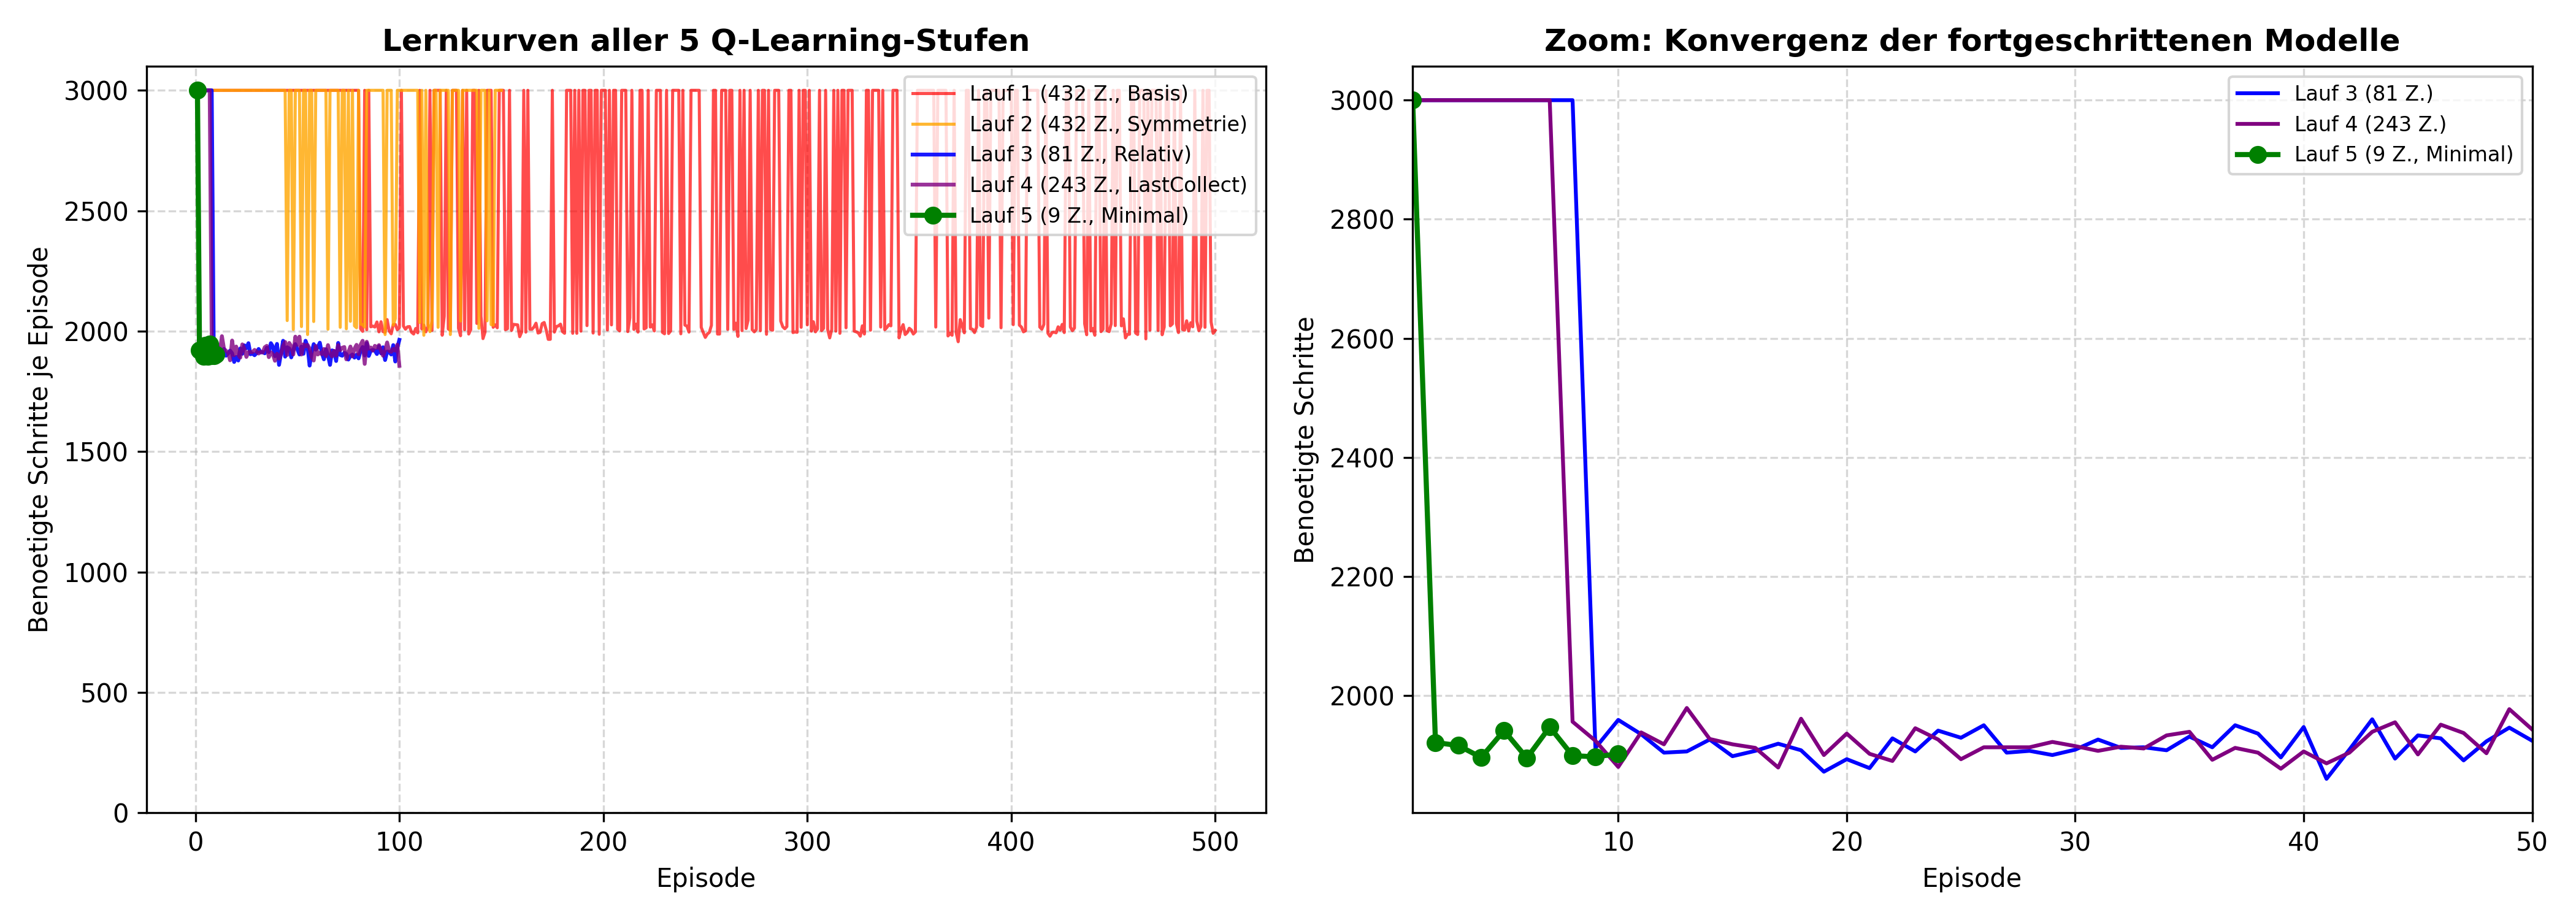
\includegraphics[width=\textwidth]{lernkurven_vergleich.png}
\caption{Lernkurven aller fünf Entwicklungsstufen (links: Gesamtlaufzeit, rechts: Detailansicht der fortgeschrittenen Modelle).}
\label{fig:lernkurven}
\end{figure}

\begin{itemize}
  \item \textbf{Lauf 1 \& 2:} Verharren über hunderte Episoden am Limit von $3.000$ Schritten. Die unzureichende Exploration seltener Zustände und der Farming-Exploit verhindern das Erreichen des Ziels.
  \item \textbf{Lauf 3 (81 Zustände):} Zeigt ab Episode 15 einen steilen Lernfortschritt und stabilisiert sich zuverlässig um $\approx 1.960$ Schritte.
  \item \textbf{Lauf 5 (9 Zustände):} Erreicht bereits in \textbf{Episode 1} einen erfolgreichen Abschluss und konvergiert nach nur 8 Episoden auf das globale Optimum.
\end{itemize}

\subsection{Der Reflex-Agenten-Hypothesentest: Mit vs. Ohne LastCollect}
Um messtechnisch zu validieren, ob das Gedächtnis (\texttt{lastcollect}) überhaupt einen theoretischen Informationsvorteil bietet, wurden zwei identisch konfigurierte Simple Reflex Agents auf derselben deterministischen Teile-Sequenz verglichen.

\begin{figure}[htbp]
\centering
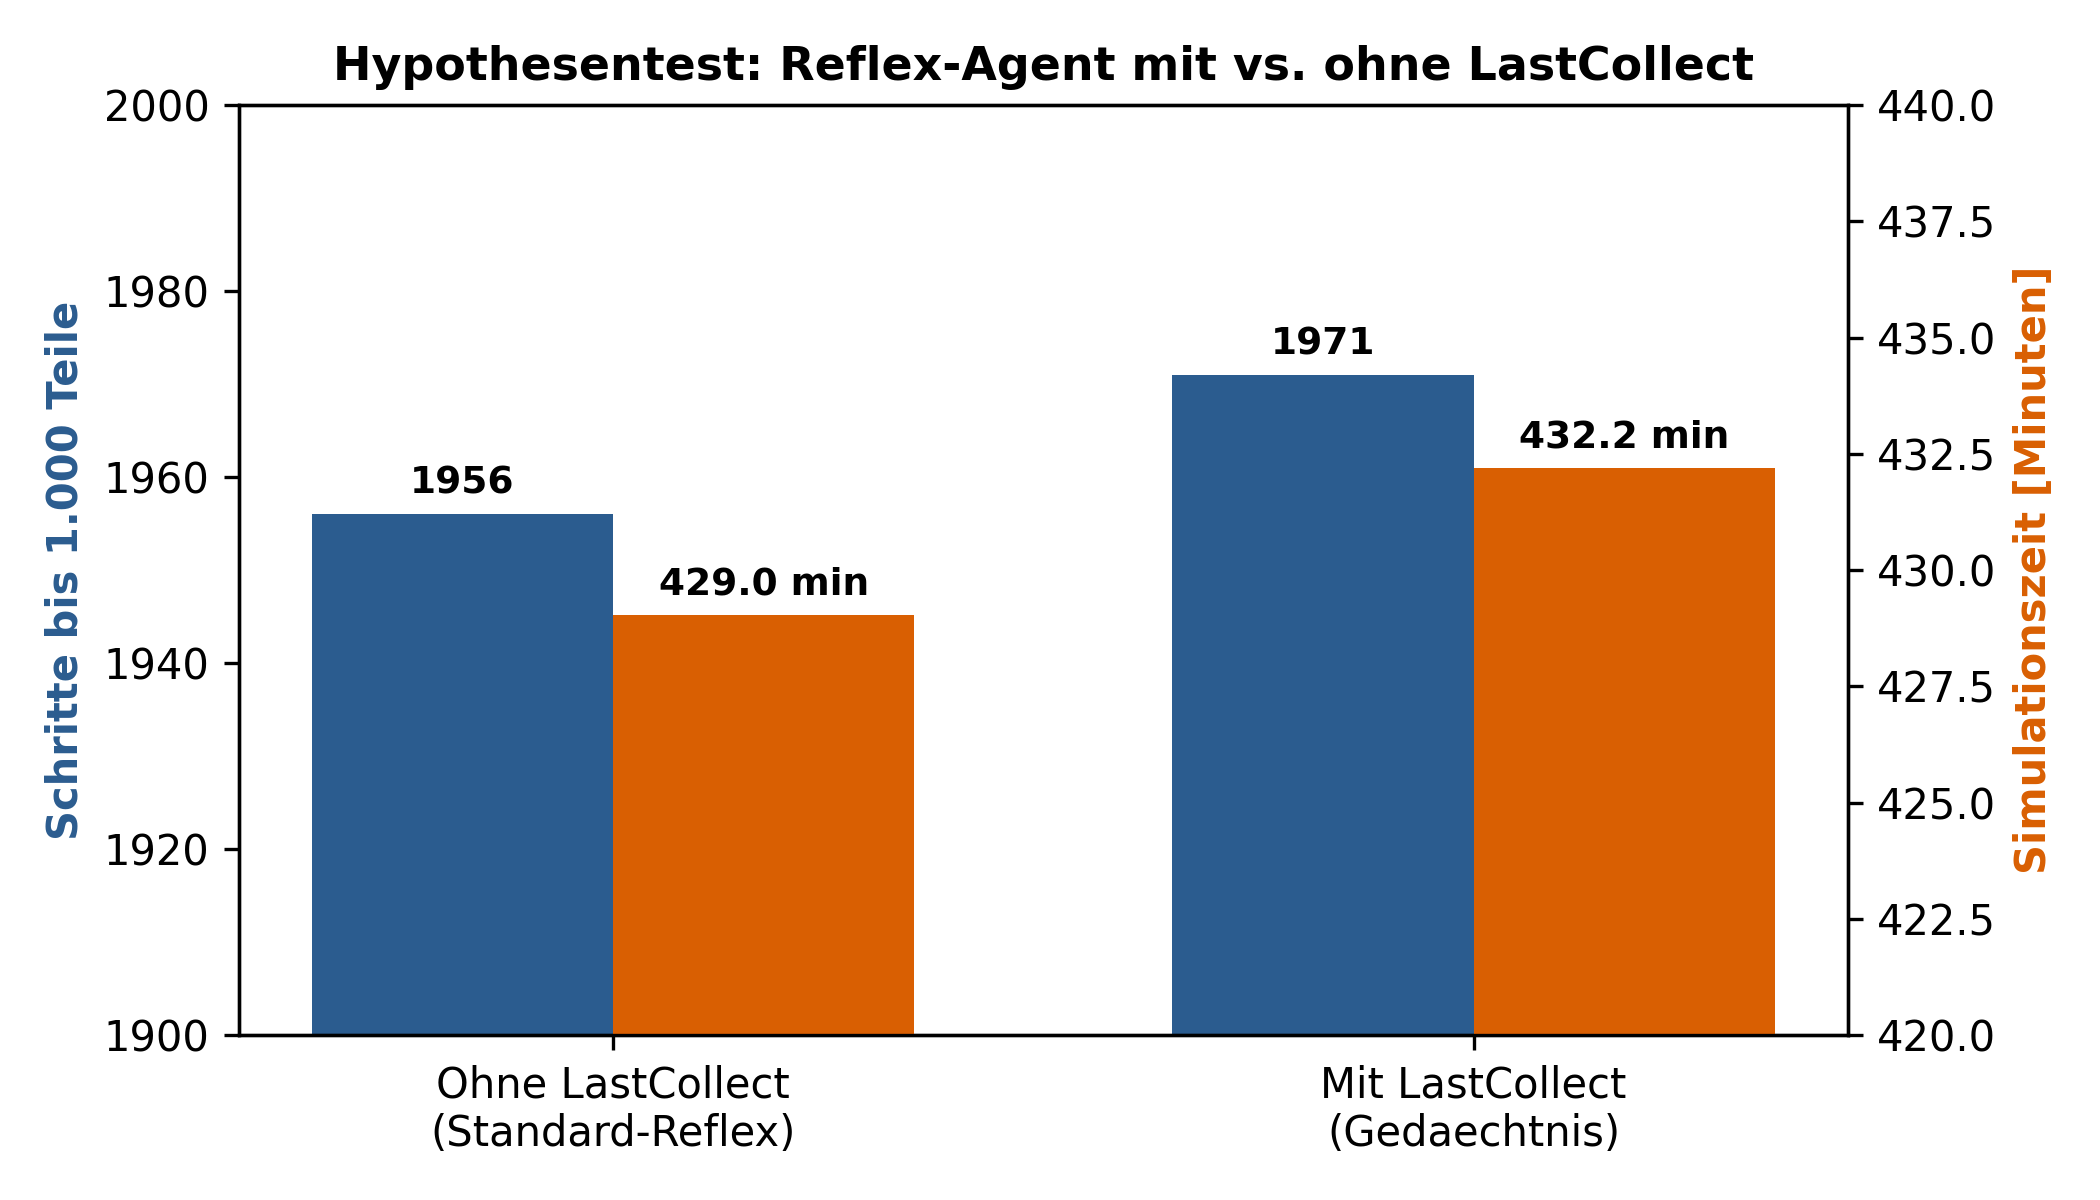
\includegraphics[width=0.75\textwidth]{reflex_vergleich.png}
\caption{Messergebnis des Hypothesentests: Reflex-Agent ohne vs. mit LastCollect.}
\label{fig:reflex_vergleich}
\end{figure}

\paragraph{Messergebnis:}
\begin{itemize}
  \item \textbf{Ohne LastCollect:} 1.956 Schritte $\mid$ Simulationszeit: \textbf{$429\text{ min } 02\text{ s}$} ($1.544.532\,\text{s}$).
  \item \textbf{Mit LastCollect:} 1.971 Schritte $\mid$ Simulationszeit: \textbf{$432\text{ min } 12\text{ s}$} ($1.555.937\,\text{s}$).
\end{itemize}
Überraschenderweise war die Variante \textbf{ohne} Gedächtnis um genau \textbf{15 Schritte ($+0{,}77\,\%$) bzw. 3 Minuten schneller}!

\paragraph{Mathematisch-stochastischer Beweis der 15 Zusatzschritte:}
Aus der Anlagenstruktur lässt sich die Differenz exakt herleiten:
\begin{enumerate}
  \item Um $1.000$ Teile in 10er-Chargen abzuführen, treten exakt $N_{\text{Drain}} = 100$ Entleerungen auf.
  \item Nach einem Drain ist genau ein Puffer leer. Das nächste Teil am Roboter stammt zu $50\,\%$ von der Schleife (fast sicher der gestaute Typ $\implies LC=2$) und zu $50\,\%$ aus dem Lager (Gleichverteilung $\frac{1}{3} \text{ Typ 1}, \frac{1}{3} \text{ Typ 2}, \frac{1}{3} \text{ Typ 3}$).
  \item Die Wahrscheinlichkeit, dass unmittelbar nach dem Drain ein frisch entleertes Teil ($LC=1$) aus dem Lager ankommt, beträgt exakt:
  \[
    P(LC=1 \mid \text{nach Drain}) = 0{,}5 \times \frac{1}{3} = \frac{1}{6} \approx \mathbf{16{,}67\,\%}
  \]
  \item Die erwartete Anzahl an Abweisungen in die Schleife ergibt sich zu:
  \[
    \mathbb{E}[\Delta \text{Schritte}] = 100 \times \frac{1}{6} \approx \mathbf{16{,}67 \text{ Schritte}}
  \]
\end{enumerate}
In genau diesen $\approx 15$ bis 17 Fällen hat der \texttt{lastcollect}-Agent das Teil unnötig in die Schleife geschickt, um auf den Stautyp zu warten. Da die Schleife eine reale Förderzeit besitzt, erzeugt jede Abweisung eine unumkehrbare Transportlatenz. Das sofortige Belegen des freien Puffers (Parallelität) ist somit physikalisch überlegen. 

\begin{center}
\fbox{\parbox{0.93\textwidth}{\textbf{Kernerkenntnis:} Dass der Q-Learning-Agent in Stufe 4 den Zustand \texttt{lastcollect} ignorierte, war \textbf{kein unvollständiges Lernen}, sondern das mathematisch und physikalisch exakte Auffinden der optimalen Policy!}}
\end{center}

\subsection{Redundanz der Puffer-Füllstände}
Analog verhält es sich mit den Füllständen ($b_1\text{cat}, b_2\text{cat}$): Da die Anti-Farming-Reward-Funktion das absichtliche Überschreiben eines belegten Puffers strikt bestraft, ist es in \textbf{keiner einzigen Situation optimal, einen belegten Puffer zu flushen}. Die Entscheidung hängt ausschließlich davon ab, ob ein Puffer frei ist ($0$), gematcht werden kann ($1$) oder blockiert ist ($2$). Die Zählerstände tragen keine Information für die optimale Aktion.

\subsection{Die finale Q-Tabelle aus Lauf 5}
Tabelle~\ref{tab:finale_q_tabelle} zeigt die vollständige, fehlerfrei auskonvergierte Q-Tabelle aus Lauf 5.

\begin{table}[htbp]
\centering
\caption{Vollständige Q-Tabelle der optimalen Policy (Lauf 5)}
\label{tab:finale_q_tabelle}
\begin{tabular}{@{}c lcc rrr c@{}}
\toprule
\textbf{Index} & \textbf{B1} & \textbf{B2} & \textbf{Situation} & \textbf{$Q(\text{P1})$} & \textbf{$Q(\text{P2})$} & \textbf{$Q(\text{Return})$} & \textbf{Optimale Aktion} \\
\midrule
0 & leer & leer & Beide leer & \textbf{610,18} & \textbf{610,18} & $-0,27$ & Puffer 1 / 2 (Sym.) \\
1 & leer & match & Match P2 & $-0,01$ & \textbf{620,33} & $-0,24$ & \textbf{Puffer 2 (Match)} \\
2 & leer & dismatch & P1 frei, P2 block & \textbf{609,81} & $-0,05$ & $-0,27$ & \textbf{Puffer 1 (Neu)} \\
3 & match & leer & Match P1 & \textbf{620,33} & $-0,01$ & $-0,24$ & \textbf{Puffer 1 (Match)} \\
4 & match & match & Beide Match & \textbf{651,59} & \textbf{651,59} & $-0,27$ & \textbf{Puffer 1 / 2} \\
5 & match & dismatch & Match P1, P2 block & \textbf{620,33} & $-0,05$ & $-0,24$ & \textbf{Puffer 1 (Match)} \\
6 & dismatch & leer & P1 block, P2 frei & $-0,05$ & \textbf{609,81} & $-0,27$ & \textbf{Puffer 2 (Neu)} \\
7 & dismatch & match & P1 block, Match P2 & $-0,05$ & \textbf{620,33} & $-0,24$ & \textbf{Puffer 2 (Match)} \\
8 & dismatch & dismatch & Beide blockiert & $-1,33$ & $-1,33$ & \textbf{689,08} & \textbf{Return-Schleife} \\
\bottomrule
\end{tabular}
\end{table}

% ======================================================================
\section{Fazit und Ausblick}
% ======================================================================

\subsection{Zusammenfassung der Ergebnisse}
Im Rahmen dieses Projekts wurde erfolgreich ein tabellarischer Q-Learning-Agent zur Optimierung eines diskreten Materialflusssystems entwickelt. Die zentralen Erkenntnisse lassen sich wie folgt zusammenfassen:
\begin{enumerate}
  \item \textbf{Zustandsraum-Kompression ($99{,}81\,\%$):} Durch den Übergang von absoluten Zählerständen ($4.800$ Zustände) auf relative Pufferrelationen ($9$ Zustände) wurde das Problem von unlösbarer Dimensionalität in ein extrem schnell konvergierendes System überführt.
  \item \textbf{Potentialerhaltendes Reward Shaping:} Ein fehlerhaft skaliertes Reward-Design führt zu unerwünschtem Reward Hacking (Farming). Die exakte Abstimmung von Aufbau-Potenzial und Verluststrafe ($-\frac{n(n+1)}{2}$) ist für die Konvergenz unverzichtbar.
  \item \textbf{Physikalisches Systemverständnis:} Die empirische und theoretische Analyse des \texttt{lastcollect}-Gedächtnisses beweist, dass das Einsparen von Puffer-Leerlaufzeiten die theoretische Stau-Vermeidung in kontinuierlichen Fördersystemen dominiert.
\end{enumerate}

\subsection{Kritische Würdigung und Ausblick}
Die Untersuchung der verschiedenen Modell- und Gedächtniskonfigurationen führt zu einer zentralen ingenieurwissenschaftlichen Erkenntnis über die Grenzen des Reinforcement Learnings in dieser Anordnung:

\begin{enumerate}
  \item \textbf{Geringe physikalische Freiheitsgrade des Gesamtsystems:} \\
  Die Struktur der Sortieranlage (zwei Puffer à 10 Plätze, drei Teiletypen, starre Rückführschleife) bietet inhärent nur sehr wenige echte, wirksame Entscheidungsfreiheiten. In nahezu allen Betriebssituationen ist die optimale Handlung durch die Gesetze des kontinuierlichen Materialflusses und die Pufferbelegung bereits eindeutig determiniert (Greedy-Match bzw. Belegen des freien Puffers).
  
  \item \textbf{Kein Mehrwert durch hochkomplexe Algorithmen (DQN / Deep RL):} \\
  Der Einsatz von komplexeren Verfahren wie \textit{Deep Q-Networks} (DQN) oder neuronalen Funktionsapproximatoren bietet für dieses System \textbf{keinerlei praktischen oder theoretischen Mehrwert} gegenüber dem einfachen tabellarischen Q-Learning. Da die optimale Policy auf dem minimalen 9-Zustände-Raum durch die tabellarische Bellman-Gleichung bereits mathematisch exakt, verlustfrei und in Rekordzeit gefunden wird, würden neuronale Netze lediglich Instabilitäten, Sampling-Ineffizienz und Rechenaufwand hinzufügen, ohne das physikalische Durchsatzlimit weiter verschieben zu können.

  \item \textbf{Durchsatzsteigerung erfordert anlagentechnische Erweiterungen:} \\
  Signifikante Leistungssteigerungen können in diesem Szenario nicht durch anspruchsvollere Lernalgorithmen erzielt werden, sondern erfordern zwingend \textbf{zusätzliche physikalische Freiheitsgrade} in der Anlagentechnik:
  \begin{itemize}
    \item \textbf{Dritter Pufferspeicher:} Ermöglicht die simultane, sortenreine Einlagerung aller drei Teiletypen, wodurch Abweisungen in die Schleife auf $0\,\%$ sinken.
    \item \textbf{Vorausschauende Sensorik (Look-Ahead):} Eine Vorab-Erkennung von mehreren nachfolgenden Teilen auf dem Zulaufband, um Pufferbelegungen vorausschauend auf Teile-Cluster abzustimmen.
    \item \textbf{Dynamische Förderbandgeschwindigkeiten:} Variable Bandgeschwindigkeiten der Rückführschleife zur gezielten Taktung des Rückstroms.
  \end{itemize}
\end{enumerate}

\end{document}
